\documentclass[10pt,twocolumn,letterpaper]{article}

\usepackage{cvpr}
\usepackage{times}
\usepackage{epsfig}
\usepackage{graphicx}
\usepackage{amsmath}
\usepackage{amssymb}

\def\cvprPaperID{1} % *** Enter the CVPR Paper ID here

\usepackage[breaklinks=true,bookmarks=false]{hyperref}

\cvprfinalcopy % Comment this line and it stop working! :(
\ifcvprfinal\pagestyle{empty}\fi

\def\httilde{\mbox{\tt\raisebox{-.5ex}{\symbol{126}}}}

% Pages are numbered in submission mode, and unnumbered in camera-ready
%\ifcvprfinal\pagestyle{empty}\fi
\setcounter{page}{1}

\graphicspath{ {./images/} } 

\sloppy

%-------------------------------------------------------------------------
%-------------------------------------------------------------------------

\begin{document}

%%%%%%%%% TITLE
\title{Convolutional Neural Network to Image Segmentation}

\author{Felipe Augusto Lima Reis\\
PUC Minas - Pontif\'icia Universidade Cat\'olica de Minas Gerais\\
R. Walter Ianni 255 - Bloco L - Belo Horizonte, MG, Brasil\\
{\tt\small falreis@sga.pucminas.br}
}

\maketitle
%\thispagestyle{empty}

%%%%%%%%% ABSTRACT
\begin{abstract}
   The ABSTRACT is to be in fully-justified italicized text, at the top
   of the left-hand column, below the author and affiliation
   information. Use the word ``Abstract'' as the title, in 12-point
   Times, boldface type, centered relative to the column, initially
   capitalized. The abstract is to be in 10-point, single-spaced type.
   Leave two blank lines after the Abstract, then begin the main text.
   Look at previous CVPR abstracts to get a feel for style and length.
\end{abstract}

%%%%%%%%% BODY TEXT
\section{Introduction}

Image segmentation refers to the partition of an image into a set of regions to cover it, to represent meaningful areas \cite{DOMINGUEZ}. In this task, it's possible to take pixels as base unit in most image processing tasks\cite{WANG201728}. Segmentation has two main objectives: the first is to decompose the image into parts for further analysis and the second one is to perform a change of representation \cite{DOMINGUEZ}.

The organization of this paper is as follows. In the next Section we discuss some related work and segmentations methods.  In Section \ref{sec:mat_metodos} its explained the method used in this paper. Then in Section \ref{sec:testes} we present an the results of the tests made for this paper and analise them. In Section 5 conclude the work.

%-------------------------------------------------------------------------
\section{Related Work} \label{sec:ref_teorico}

Superpixels are the result of perceptual grouping of pixels, or seen the other way around, the results of an image oversegmentation \cite{WANG201728}. One example of oversegmentation can be seen in Figure \ref{fig:superpixel}. Superpixel can cause substantial speed-up of subsequent processing since the number of superpixels of an image reduces in contrast with the original number of pixels \cite{WANG201728}.
 
\begin{figure}[ht]
  \centering
  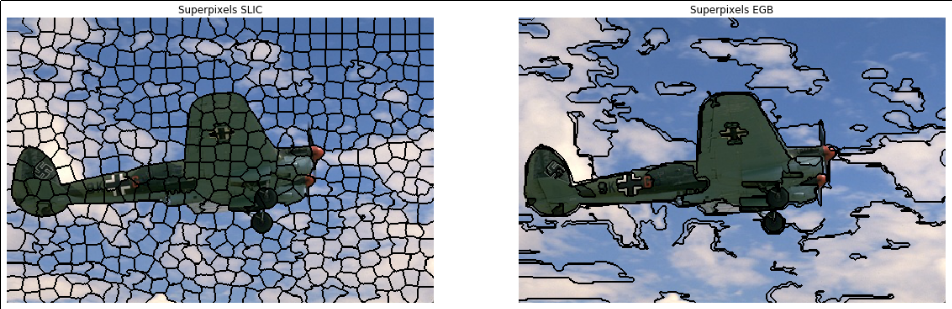
\includegraphics[width=0.48\textwidth]{superpixels.png}
  \caption{Segmented images using SLICO and EGB superpixels}
  \label{fig:superpixel}
\end{figure}

%-------------------------------------------------------------------------
\section{Segmentation Method} \label{sec:mat_metodos}

%-------------------------------------------------------------------------
\section{Tests and Results} \label{sec:testes}

%-------------------------------------------------------------------------
\section{Conclusion} \label{sec:conclusao}

%-------------------------------------------------------------------------

{\small
\bibliographystyle{ieee}
\bibliography{egbib}
}

\end{document}
